% !TeX root = ../../Thesis.tex
\chapter{Methods}
\label{chp:methods}
 
Many of the diagnostics presented in this chapter have been adapted from a large repository of LPI diagnostics for EPOCH which was created by Alexander Seaton (\href{https://orcid.org/0000-0001-5032-8918}{ORCID: 0000-0001-5032-8918}) as part of his PhD project ``Particle-in-cell Simulations of Laser-Plasma Instabilities in Shock-Ignition". Since Alex left Warwick in September 2019, I have become the main developer and maintainer for the repository.

This chapter introduces the reader to the particle-in-cell code EPOCH, which is used to perform all the simulations presented in this thesis. We also explain the methods used to turn EPOCH's output into diagnostics better-suited to the problem of stimulated Raman scattering in the kinetic regime. 

\section{The particle-in-cell method}
The core components of a PIC code are: a fixed spatial grid; a solver that moves charged particles according to the Lorentz force law and calculates currents due to this motion (the particle pusher); and a solver which uses the calculated currents to solve Maxwell's equations on the grid (the field solver) \citep{Arber2015}. There are three fundamental features of a PIC code which make it ontologically different from a true plasma: firstly, time is discrete rather than continuous; secondly, electromagnetic fields only take well-defined values on a discrete spatial grid; and thirdly, simulation pseudo-particles have a non-zero size and shape. These are computational limitations, but also practical considerations which make the mathematics behind the simulation more tractable.


\subsection{Field solver}
The key point of a PIC simulation is that the system evolves \emph{self-consistently}, this means that every time the particles move we must calculate the electric and magnetic fields generated by their new charge and current densities. To calculate these new fields we need to solve Maxwell's equations:

\begin{equation}\label{Maxwell}
\begin{aligned} 
    \nabla \times \mathbf{E} &= - \frac{\partial}{\partial t}\mathbf{B} \\
    \nabla \times \mathbf{B} &= \mu_0 \left (\mathbf{j} + \epsilon_0\frac{\partial}{\partial t}\mathbf{E}\right)\\
    \nabla \cdot \mathbf{B} &= 0\\
    \nabla \cdot \mathbf{E} &= \frac{\rho}{\epsilon_0}
\end{aligned}
\end{equation} where $\rho$ and $\mathbf{j}$ are the charge and current densities respectively, which have been calculated as part of the particle pusher. These are differential equations, which means we can solve them by some sort of finite-difference method, in which the full and partial differentials are replaced by difference equations (we saw this already in the construction of the particle pusher). The system can be simplified by realising that, since we will be solving at a discrete time step, $\partial \mathbf{B}/\partial t = \partial \mathbf{E}/\partial t =0$. This reduces the system to be solved to a single equation: 
\begin{equation}\label{Poisson}
    \bm{\nabla}^2 \phi = - \frac{\rho}{\epsilon_0}
\end{equation} which is then solved by taking Fourier transforms of $\rho$ and $\phi$. The Fourier transform is a generalisation of the complex Fourier series when the length of the function domain tends to infinity \citep{wolfram}. The Fourier transform is often thought of as a transformation between a function in the space-domain and the same function in the frequency-domain. As such, it can be defined by the functor $\mathcal{F}_x$ defined by
\begin{equation}\label{FT}
\begin{aligned}
    F(k)&=\mathcal{F}_x\left[f(x)\right](k)\\
    &= \int_{-\infty}^{\infty} f(x)e^{-2\pi i kx}dx.
\end{aligned}
\end{equation} The Fourier transform transforms $\bm{\nabla}^2$ to $k^2$, which makes Equation \ref{Poisson}
\begin{equation}
    \phi(k)=\frac{\rho (k)}{\epsilon_0 k^2},
\end{equation} this is an explicit expression for $\phi(k)$ in terms of known quantities. We can now use the inverse Fourier transform to calculate $\phi(x)$ and $\mathbf{E}(x)$ like so \citep{Birdsall}:
\begin{equation*}
    \rho(x)\xrightarrow[\text{FFT}]{}\rho(k)\xrightarrow[{k^2}]{}\phi(k)\xrightarrow[\text{IFFT}]{}\phi(x)\xrightarrow[{\nabla\phi}]{}\mathbf{E}(x)
\end{equation*}

We now have an expression for $\mathbf{E}$ on the grid, and can find $\mathbf{B}$ by substituting it back into Maxwell's equations. The final step of the field solver in EPOCH is to interpolate from the field values on the grid, to forces at the particle positions.



\subsection{Interpolation to particles}
\subsection{Particle push}
The basic particle pusher acts to integrate the equations of motion for the charged particles and then to accelerate the particles to new velocities, and to translate them to new positions. The equation of motion for charged particles in a plasma comes from the Lorentz force law:
\begin{equation} \label{lorentz}
m \frac{d\mathbf{v}}{dt} = q \left( \mathbf{E} + \mathbf{v} \times \mathbf{B} \right)
\end{equation}
In EPOCH the particle pusher actually solves the full relativistic Lorentz force law, but we will consider the non-relativistic case here for simplicity. Equation \ref{lorentz} can be solved by solving the three simultaneous equations which come from time-centering the magnetic term \citep{Birdsall} like so 
\begin{eqnarray*} \label{timecentred}
\frac{\mathbf{v}_{t+\Delta t/2}-\mathbf{v}_{t-\Delta t/2}}{\Delta t}=\frac{q}{m}\left[\mathbf{E}_t+\frac{\mathbf{v}_{t+\Delta t/2}+\mathbf{v}_{t-\Delta t/2}}{2} \times \mathbf{B}_t\right]
\end{eqnarray*} A more elegant solution is to separate solving the magnetic and electric effects on the motion by using the Boris substitution \citep{Birdsall}
\begin{equation}
\mathbf{v}_{t+\Delta t/2} = \mathbf{v}^{+}+\frac{q\mathbf{E}_t}{m}\frac{\Delta t}{2}
\label{eqhalfE}
\end{equation}
\begin{equation}
\mathbf{v}_{t-\Delta t/2} = \mathbf{v}^{-}-\frac{q\mathbf{E}_t}{m}\frac{\Delta t}{2}
\label{eqhalfE2}
\end{equation}

which gives:

\begin{equation}
\frac{\textbf{v}^{+} - \textbf{v}^{-}}{\Delta t} = \frac{q}{2m} \left( \textbf{v}^{+} + \textbf{v}^{-} \right) \times \textbf{B}_{t}.
\label{eq:c2.2}
\end{equation} The second equation of motion ($\mathbf{v}=d\mathbf{x}/dt)$ is solved using the following integrator:
\begin{equation}
    \frac{\mathbf{x}_{t+1}-\mathbf{x}_t}{\Delta t} =\mathbf{v}_{t+\Delta t/2}.
\label{dxdt}
\end{equation} Equations \ref{eq:c2.2} and \ref{dxdt} together form a second order leapfrog integrator; conventionally understood to be the integrator with the best balance between accuracy, stability and efficiency. The final step of the particle pusher is interpolating from the new particle positions and velocities to new values of the current and charge densities on the grid.
\subsection{Interpolation to the grid}
\subsection{EPOCH}
EPOCH is a collisionless plasma physics simulation code that uses the Particle in Cell (PIC) method to move particles in self-consistently evolving electric and magnetic fields. EPOCH is an MPI parallelised, explicit, second-order, relativistic PIC code which is controlled through a customisable input deck \cite{Arber2015}.
 The interaction of the user with the EPOCH code is limited to the creation of an input deck for each simulation experiment. This document contains the key simulation parameters, such as: the charge and density of various particle species; background electric and magnetic fields; and the duration of the simulation. The input deck also requires you to choose the sizes of your spatial grid and time step, this is very important as you need to be able to resolve the effect you are studying.
 
``EPOCH (Extendable PIC Open Collaboration) project. EPOCH is a Birdsall and Langdon (with Villasenor and Buneman charge conservation) type Particle in Cell (PIC) code in 1, 2 and 3D that has been developed at the University of Warwick as the basis for a standard, extendable PIC code. It has been designed for both ease of use and ease of extension with both new physics and new user interface elements. EPOCH is written using standard Fortran95 and MPI and is open source enabling it to be easily modified for specic use cases. The code has seen widespread adoption with several hundred registered users and has become one of the standard PIC codes used by the plasma physics research community." Keith's website



\section{EPOCH benchmarking}
\subsection{Dispersion relations}
\subsection{Linear growth rates}



\section{Diagnostics}



The EPOCH code produces outputs in terms of physical variables, for example, electric and magnetic fields as functions of space and time. It can be useful to plot these directly.

\subsection{Frequency-filtered diagnostics}
The core element of several diagnostics used in this thesis is the ability to separate the $E_y$ and $B_z$ fields into different frequency components. 

\subsubsection{Bandstop filter for scattered light} When SRS is measured in experiments, the value reported is the reflectivity: the ratio of SRS-scattered light to incident laser light. In order to measure this in our simulations, we use a bandstop filter to separate out the contributions of SRS-scattered light from any other light which might travel backwards through the laser-entry boundary. Figure \ref{fig:bandstop} shows a typical electromagnetic frequency spectrum for the simulations considered in Chapter \ref{chp:iSRS}. The red-shaded band represents the filter bandwidth of $0.3\omega_0$. We choose a filter length of 1001, to achieve a reasonable balance between computation time and the transition bandwidth. Finally, we create a sinc filter kernel which is then multiplied by a Hamming window to create a \textit{windowed-sinc filter}. After filtering the $E_y$ and $B_z$ signals to remove all frequency contributions in the red band, we compute the Poynting flux through the left boundary by: $S(t)=E_yB_z/\mu_o$.


\begin{figure}[ht]
   \centering
    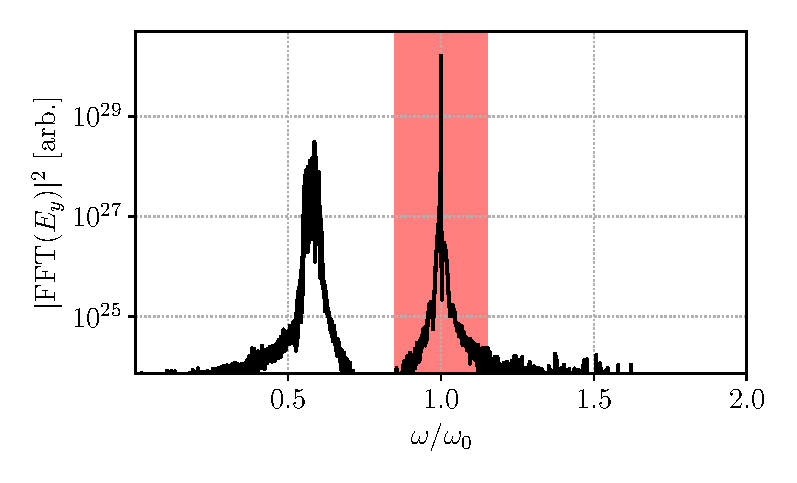
\includegraphics[width=0.8\columnwidth]{Chapters/C3_Methods/EyFFT1D_filter_bandwidth.pdf}
    \caption{Fourier-transform of $E_y(t)$ at laser-entry boundary (back-scattered light exit boundary). Before the application of the bandstop filter, we see two peaks: the peak at 1.0 is the incident laser, and the broader peak around 0.55 is the light scattered by SRS. The red shaded area represents the bandwidth of frequencies that will be attenuated by our filter.}
    \label{fig:bandstop}
\end{figure}{}

\subsection{Inflation threshold diagnostic}\label{diag:threshold}

This diagnostic 

According to fluid theory, the growth of a parametrically unstable mode in an inhomogeneous plasma is limited by the loss of resonance between the waves as they propagate through the plasma and experience wave-number shift \cite{Rosenbluth1972}. We can formulate this inhomogeneous growth in terms of the Rosenbluth gain exponent\cite{Rosenbluth1972}
\begin{equation}\label{eqn:GRos}
    G_\mathrm{Ros} = 2\pi\gamma_0^2/|v_{g,1}v_{g,2}\kappa'|,
\end{equation}
where $\gamma_0$ is the growth rate of the equivalent mode in a homogeneous plasma, $v_{g,1}, v_{g,2}$ are the group speeds of the scattered EM wave/EPW and $\kappa'$ is the $x$-derivative of the wave-number mismatch $\kappa(x) = k_0(x) -k_\mathrm{s}(x) -k_\mathrm{EPW}(x)$. The maximum intensity reached by a parametrically unstable wave which has grown from noise at point $x$ is then given by the expression $I_\mathrm{noise}\mathrm{exp}(G_\mathrm{Ros}(x))$. In order to calculate the intensity of scattered light due to SRS, we substitute for $k_0,k_\mathrm{s},k_\mathrm{EPW}$ using the electromagnetic and Bohm-Gross dispersion relations in one dimension, to get:
\begin{equation}\label{eqn:kappaPrime}
    \frac{d\kappa}{dx}= -\frac{1}{2}\frac{q_e^2}{m_e\epsilon_0}
    \left(\frac{1}{c^2k_0}-\frac{1}{3v_\mathrm{th}^2k_\mathrm{EPW}}-\frac{1}{c^2k_\mathrm{s}}\right)\frac{dn_e}{dx}.
\end{equation}
Substituting this back into $G_\mathrm{Ros}$ with the growth rate for backward SRS in a homogeneous plasma\cite{kruer2003},
\begin{equation}\label{eqn:gamma0}
    \centering
    \gamma_0 = \frac{k_\mathrm{EPW}v_{os}}{4}\left[\frac{\omega_{\mathrm{pe}}^2}{\omega_\mathrm{EPW}(\omega_0-\omega_\mathrm{EPW})}\right]^{1/2},
\end{equation}
gives an appropriate Rosenbluth gain exponent for calculating convective amplification of
back-scattered SRS light in our simulations.


We make several simplifying assumptions that allow us to estimate the maximal scattered light intensity at a point in our simulation domain. Firstly, we neglect the dependence of the scattered light velocity on space, and consider it to be fixed at $c$. This means that we slightly over-estimate the amount of scattered light which is able to reach the point $x$ in time $t$. We also assume that the laser achieves its maximum intensity starting at $t=0$ rather than ramping up, as it does in the simulations.
We neglect collisional damping of the scattered EM waves and assume that the noise source $I_\mathrm{noise}$ is homogeneous in the domain. Finally, we assume that the amplification described by the Rosenbluth gain exponent occurs locally and instantaneously at the point of perfect
matching $(\kappa=0)$, rather than across the resonance region defined by $\ell \sim 1/\sqrt{\kappa'}$. For all the simulations presented in this paper $\ell < 6\si{\micro\metre}$.
 The scattered light intensity is then given by
 \begin{equation}\label{eqn:fluid_model}
     I(x) = \frac{1}{L_x}\int_x^{L_x}I_\mathrm{noise}\mathrm{exp}(G_\mathrm{Ros}(s)) ds.
 \end{equation}
The prefactor $1/L_x$ ensures that if $G_\mathrm{Ros}=0$, such that there is no growth, then the back-scattered signal remains
at the the noise intensity. The steady-state intensity of SRS scattered light measured at the laser-entry boundary is then given by $\langle I_{\mathrm{SRS}} \rangle = I(0)$.

Obviously this model is limited to calculating the maximum reflected light ignoring the effects of pump depletion.  It is only applicable for these intensities ... . Using the code LPSE might be more realistic, but we don't think it can do convective growth yet. In Han braodband preprint they find the trheshold by fitting some weird function, what do I think of that?

%\bibliographystyle{plainnat}
%\bibliography{Chapters/C3_Methods/Methods}
